%!TEX root = ../../book_ML.tex
\chapter{Máy vector hỗ trợ}
% \chapter{Support vector machine}
\label{cha:svm}
% Trong loạt bài tiếp theo, tôi sẽ trình bày về một trong những thuật toán classification phổ biến nhất (cùng với \href{http://machinelearningcoban.com/2017/02/17/softmax/}{softmax regression}). Có rất nhiều suy luận toán học trong phần này yêu cầu bạn cần có kiến thức về \href{http://machinelearningcoban.com/2017/04/02/duality/}{Duality} cũng như về tối ưu lồi. Bạn được khuyến khích đọc các Bài 16, 17, và 18 trước khi đọc bài này.  
\index{máy vector hỗ trợ -- support vector machine}

% \textit{Nếu không muốn đi sâu vào phần toán, bạn có thể bỏ qua Mục \ref{sec:19_svm3}.} 


\section{Giới thiệu}
\textit{Máy vector hỗ trợ} (support vector machine, SVM) là một trong những
thuật toán phân loại phổ biến và hiệu quả. Ý tưởng đứng sau SVM khá đơn giản,
nhưng để giải bài toán tối ưu SVM, chúng ta cần kiến thức về tối ưu và đối ngẫu.

Trước khi đi vào phần ý tưởng chính của SVM, chúng ta cùng ôn lại kiến thức về hình học giải tích trong chương trình phổ thông. 
 
 
\subsection{Khoảng cách từ một điểm tới một siêu mặt phẳng}
Trong không gian hai chiều, khoảng cách từ một điểm có toạ độ $(x_0, y_0)$ tới
{đường thẳng} có phương trình $w_1x + w_2y + b = 0$ được xác định bởi
\begin{equation*} 
\frac{|w_1x_0 + w_2y_0 + b|}{\sqrt{w_1^2 + w_2^2}} 
\end{equation*} 
Trong không gian ba chiều, khoảng cách từ một điểm có toạ độ $(x_0, y_0, z_0)$ tới một {mặt phẳng} có phương trình $w_1x + w_2y + w_3 z + b = 0$ được xác định bởi
\begin{equation*} 
\frac{|w_1x_0 + w_2y_0 + w_3z_0 + b|}{\sqrt{w_1^2 + w_2^2 + w_3^2}} 
\end{equation*} 
Hơn nữa, nếu bỏ dấu trị tuyệt đối ở tử số, ta có thể xác định được điểm
đó nằm về phía nào của {đường thẳng} hay {mặt phẳng} đang xét.
Những điểm làm cho biểu thức trong dấu trị tuyệt đối mang dấu dương nằm về
cùng một phía (tạm gọi là \textit{phía dương}), những điểm làm
cho giá trị này mang dấu âm nằm về phía còn lại (gọi là \textit{phía âm}). Những điểm làm cho tử số bằng không sẽ nằm trên đường thẳng/mặt phẳng phân chia.

Các công thức này có thể được tổng quát lên cho trường hợp không gian $d$ chiều.
Khoảng cách từ một điểm (vector) có toạ độ $(x_{10}, x_{20}, \dots, x_{d0})$ tới
{siêu phẳng} $w_1x_1 + w_2x_2 +
\dots + w_dx_d   + b = 0$ được xác định bởi
\begin{equation*} 
\frac{|w_1x_{10} + w_2x_{20} + \dots +
w_dx_{d0} + b|}{\sqrt{w_1^2 + w_2^2 + \dots +
w_d^2}} = \frac{|\mathbf{w}^T\mathbf{x}_0 + b|}{\|\mathbf{w}\|_2}
\end{equation*} 
với $\bx_0 = [x_{10}, x_{20}, \dots, x_{d0}]^T, \bw = [w_1, w_2,
\dots, w_d]^T$.
 
 
\subsection{Nhắc lại bài toán phân loại hai lớp dữ liệu}
 
Xin nhắc lại bài toán phân loại đã đề cập trong
Chương~\ref{cha:pla} (PLA). Giả sử có hai
lớp dữ liệu được mô tả bởi các vector đặc trưng trong không gian nhiều
chiều. Hơn nữa, hai lớp dữ liệu này là tách biệt tuyến tính, tức tồn
tại một siêu phẳng phân chia chính xác hai lớp đó. Hãy tìm một siêu phẳng sao cho tất cả các điểm thuộc một lớp nằm về cùng một
phía của siêu phẳng đó và ngược phía với toàn bộ các điểm thuộc lớp còn lại.
Chúng ta đã biết rằng, thuật toán PLA có thể thực hiện được việc này nhưng PLA có thể cho vô số nghiệm như Hình~\ref{fig:19_linsep}.
 
% ******************************************************************************
\begin{figure}[t]
    % caption on side     
    \floatbox[{\capbeside\thisfloatsetup{capbesideposition={right, top},capbesidewidth=6cm}}]{figure}[\FBwidth]
    {\caption[]{Hai lớp dữ liệu vuông và tròn là tách biệt tuyến tính. Có
    vô số đường thằng có thể phân loại chính xác hai lớp dữ liệu này (xem
    thêm Chương~\ref{cha:pla}).}
    \label{fig:19_linsep}}
    {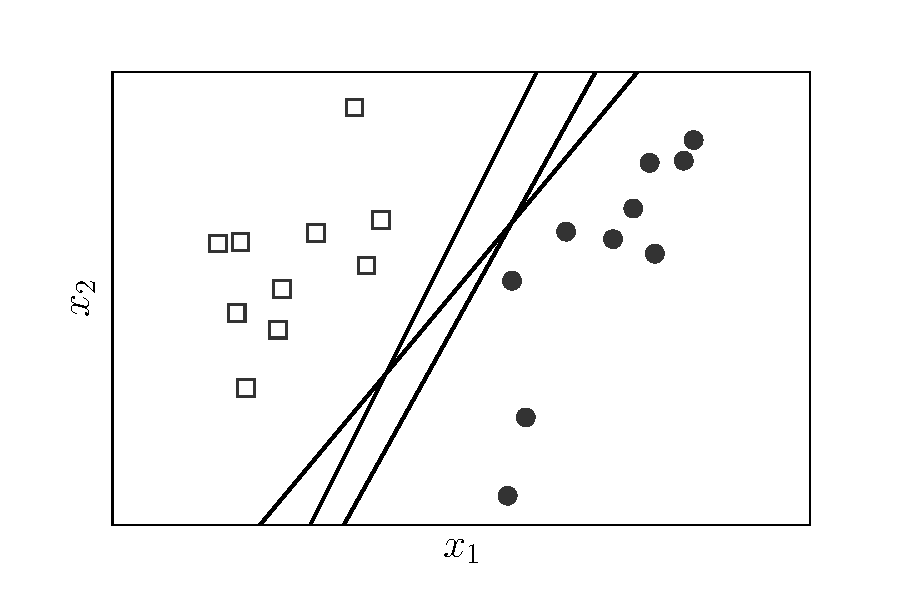
\includegraphics[width = .5\textwidth]{ebookML_src/src/svm/svm1.pdf}}
    % \myrule
\end{figure}
% ******************************************************************************

Có một câu hỏi được đặt ra: Trong vô số các mặt phân chia đó, đâu là mặt
tốt nhất? Trong ba đường thẳng minh họa trong Hình~\ref{fig:19_linsep}, có hai
đường thẳng khá lệch về phía lớp hình tròn. Điều này có thể khiến nhiều điểm hình tròn chưa nhìn thấy bị phân loại lỗi thành điểm hình vuông. Liệu có
cách nào tìm được đường phân chia sao cho đường này không lệch về một lớp không? 

Để trả lời câu hỏi này, chúng ta cần tìm một tiêu chuẩn để đo sự \textit{lệch} về mỗi lớp của đường phân chia. 
% ******************************************************************************
\begin{figure}[t]
    \begin{subfigure}{0.49\textwidth}
    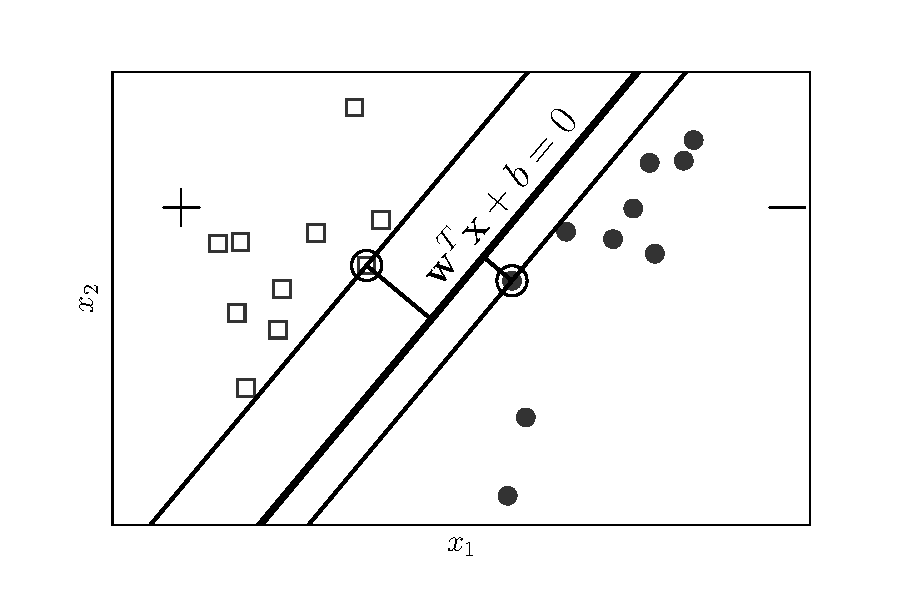
\includegraphics[width=0.99\linewidth]{ebookML_src/src/svm/svm2.pdf}
    \caption{}
    % \label{fig:subim1}
    \end{subfigure}
    \begin{subfigure}{0.49\textwidth}
    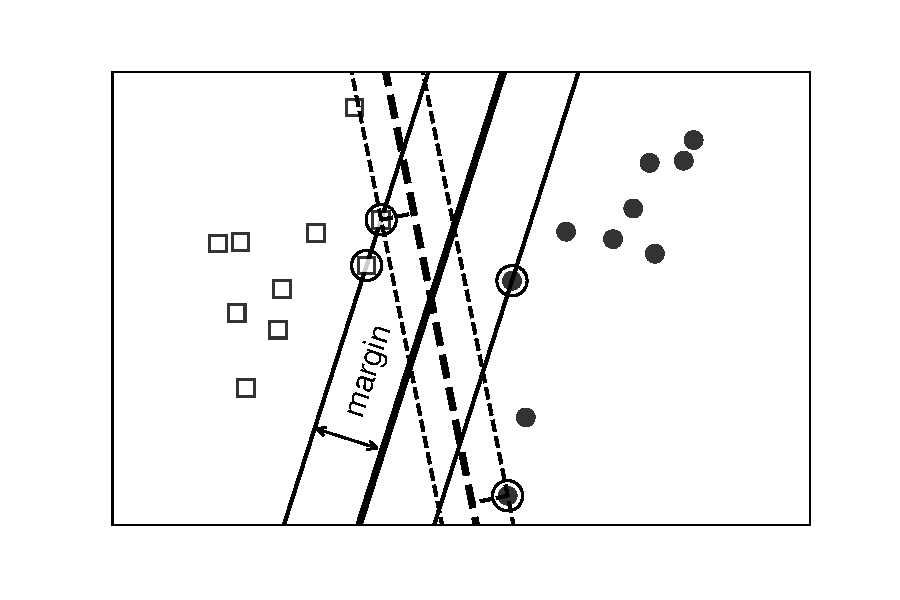
\includegraphics[width=0.99\linewidth]{ebookML_src/src/svm/svm5.pdf}
    \caption{}
    % \label{fig:subim2}
    \end{subfigure}
    \caption{Ý tưởng của SVM. Lề của một lớp được
 định nghĩa là khoảng cách từ các điểm gần nhất của lớp đó tới mặt phân
    chia. Lề của hai lớp phải bằng nhau và lớn nhất có thể.}
    \label{fig:19_svm2}
\end{figure}
% ******************************************************************************
\index{máy vector hỗ trợ -- support vector machine!lề -- margin}
\index{bộ phân loại lề rộng nhất -- maximum margin classifier}
Gọi khoảng cách nhỏ nhất từ một điểm thuộc một lớp tới đường phân chia là \textit{lề} (margin). Ta cần tìm một đường phân chia sao cho lề của hai lớp là như nhau đối với đường phân chia đó. Hơn nữa, độ rộng của lề càng lớn thì khả năng xảy ra phân loại lỗi càng thấp. Bài toán tối ưu trong SVM chính là bài toán đi tìm đường phân chia
sao cho lề rộng nhất. Đây cũng là lý do SVM
còn được gọi là \textit{bộ phân loại lề lớn nhất} ({maximum margin classifier}). Nguồn gốc tên gọi
\textit{máy vector hỗ trợ} sẽ sớm được làm sáng tỏ.
 

 
% Để giúp các bạn dễ hình dung, chúng ta cùng xét trường hợp trong không gian hai
% chiều dưới đây. \textit{Không gian hai chiều để các bạn dễ hình dung, các phép
% toán hoàn toàn có thể được tổng quát lên không gian nhiều chiều.}
 


% %% *****************************************************************************
% \begin{figure}[t]
%     \begin{subfigure}{0.495\textwidth}
%     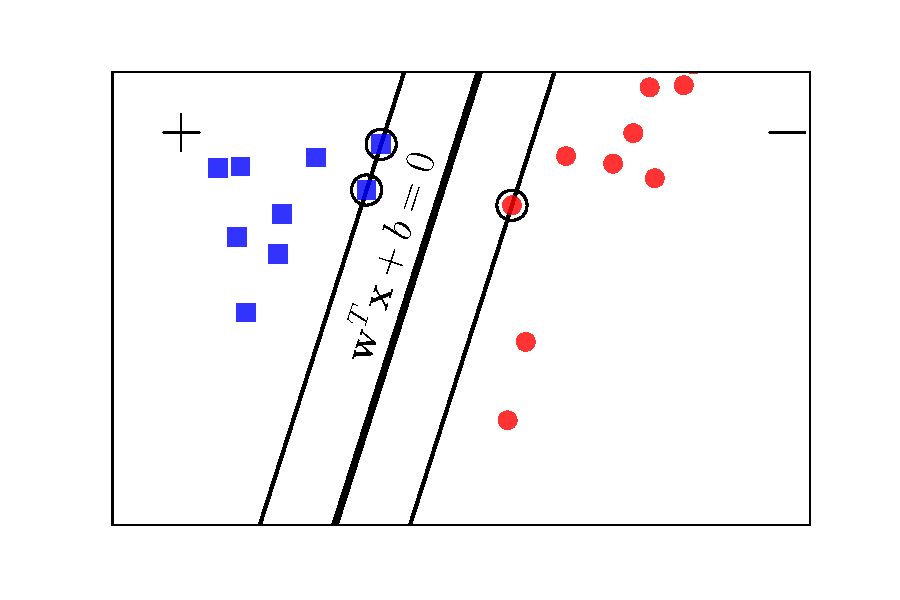
\includegraphics[width=\linewidth]{ebookML_src/src/svm/svm6.pdf}
%     \caption{}
%     \label{fig:svmf3a}
%     \end{subfigure}
%     \begin{subfigure}{0.495\textwidth}
%     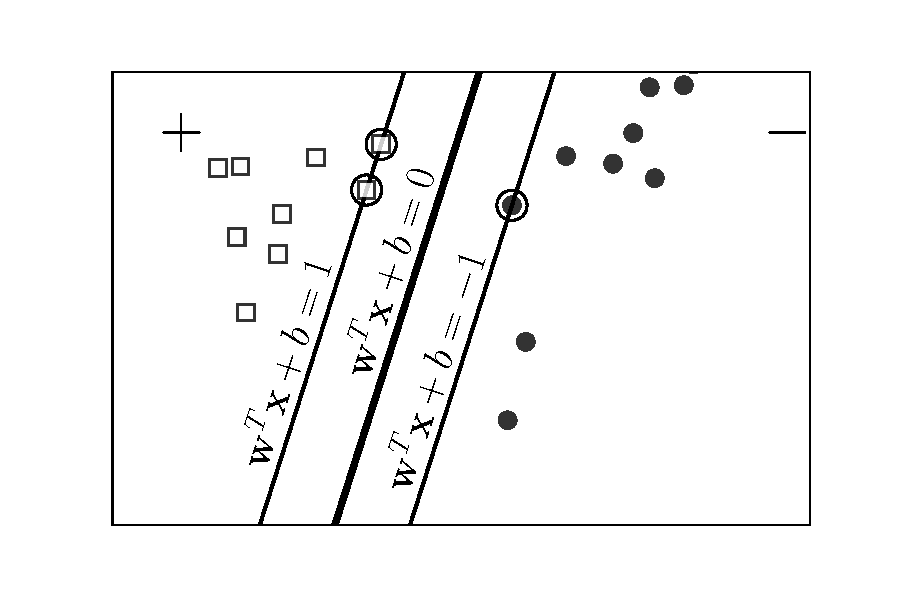
\includegraphics[width=\linewidth]{ebookML_src/src/svm/svm3.pdf}
%     \caption{}
%     \label{fig:svmf3b}
%     \end{subfigure}
%     \caption{
%      Phân tích bài toán SVM. 
%     }
%     \label{fig:svmf3}
% \end{figure}
% ******************************************************************************
%% *****************************************************************************

% ******************************************************************************
 
% Để dễ hình dung, chúng ta cùng làm với các ví dụ trong không gian hai chiều. 
\section{Xây dựng bài toán tối ưu cho máy vector hỗ trợ} 
Giả sử dữ liệu trong tập huấn luyện là các cặp (vector đặc trưng, nhãn): $(\mathbf{x}_1, y_1),
(\mathbf{x}_2, y_2), \dots, (\mathbf{x}_N, y_N)$ 
{nhãn} bằng +1 hoặc -1 và $N$ là số điểm dữ liệu.
Không mất tính tổng quát, giả sử các điểm vuông có nhãn là 1, các điểm tròn có nhãn là -1 và siêu phẳng $\mathbf{w}^T\mathbf{x} + b  = 0$ là mặt phân chia hai lớp (Hình~\ref{fig:svmf3}). Ngoài ra, lớp hình vuông nằm về {phía
dương}, lớp hình tròn nằm về {phía âm} của mặt phân chia. Nếu  xảy ra điều ngược lại, ta
chỉ cần đổi dấu của $\mathbf{w}$ và $b$. Bài toán tối ưu trong SVM sẽ là bài toán đi tìm các tham số mô hình $\bw$ và $b$.
%%
% *****************************************************************************D
  \begin{figure}[t]
    % caption on side     
    \floatbox[{\capbeside\thisfloatsetup{capbesideposition={right,top},capbesidewidth=6cm}}]{figure}[\FBwidth]
    {\caption{Giả sử mặt phân chia có phương trình $\bw^T\bx+b = 0$. Không mất
    tính tổng quát, bằng cách nhân các hệ số $\bw$ và $b$ với các hằng số phù
    hợp, ta có thể giả sử rằng điểm gần nhất của lớp vuông tới
    mặt này thoả mãn $\bw^T\bx + b = 1$. Khi đó, điểm gần nhất của lớp tròn
    thoả mãn $\bw^T\bx + b = -1$.}
    \label{fig:svmf3}}
    {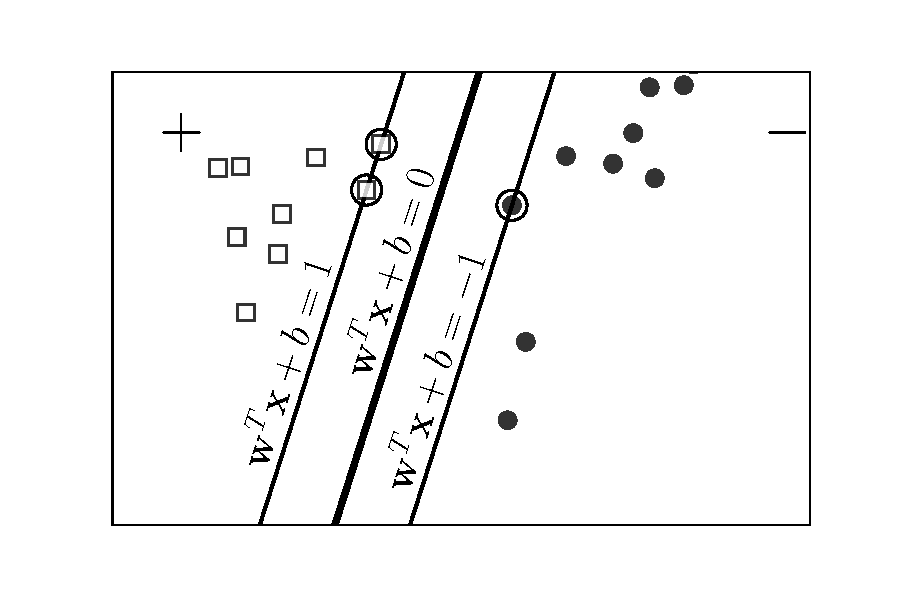
\includegraphics[width=7.5cm]{ebookML_src/src/svm/svm3.pdf}}
    % \myrule
\end{figure}
% *****************************************************************************D

Với cặp dữ liệu 
$(\mathbf{x}_n, y_n)$ bất kỳ, khoảng cách từ $\bx_n$ tới mặt phân chia là
\begin{math} 
\frac{y_n(\mathbf{w}^T\mathbf{x}_n + b)}{\|\mathbf{w}\|_2} 
\end{math}. 
Điều này xảy ra ta đã giả sử $y_n$ cùng dấu với {phía} của $\mathbf{x}_n$. Từ đó suy ra $y_n$ cùng dấu với
$(\mathbf{w}^T\mathbf{x}_n + b)$ và tử số luôn là một đại lượng không âm.
Với mặt phân chia này, lề được tính là khoảng cách gần nhất từ một
điểm (trong cả hai lớp, vì cuối cùng lề của hai lớp bằng nhau)
tới mặt phân chia:
\begin{equation*} 
\text{lề} = \min_{n} \frac{y_n(\mathbf{w}^T\mathbf{x}_n + b)}{\|\mathbf{w}\|_2} 
\end{equation*} 
Bài toán tối ưu của SVM đi tìm $\mathbf{w}$ và $b$ sao cho lề đạt giá trị lớn nhất: 
\begin{equation} 
\label{eqn:19_svm1}
(\mathbf{w}, b) = \arg\max_{\mathbf{w}, b} \left\{ 
    \min_{n} \frac{y_n(\mathbf{w}^T\mathbf{x}_n + b)}{\|\mathbf{w}\|_2}  
\right\} 
= \arg\max_{\mathbf{w}, b}\left\{ 
    \frac{1}{\|\mathbf{w}\|_2} \min_{n} y_n(\mathbf{w}^T\mathbf{x}_n + b) 
\right\}
\end{equation} 
Nếu ta thay vector trọng số $\mathbf{w}$ bởi
$k\mathbf{w}$ và $b$ bởi $kb$ trong đó $k$ là một hằng số dương {bất kỳ}
thì mặt phân chia không thay đổi, tức khoảng cách từ từng điểm đến mặt phân chia
không đổi, tức lề không đổi. Vì vậy, ta có thể giả
sử:
\begin{equation*} 
y_m(\mathbf{w}^T\mathbf{x}_m + b) = 1 %\Leftrightarrow \bw^T\bx_m + b = 1
\end{equation*} 
{với những điểm nằm gần mặt phân chia nhất} (được khoanh tròn trong Hình \ref{fig:svmf3}).
% chúng là các điểm được khoanh tròn. 

Như vậy, với mọi $n$ ta luôn có 
\begin{equation*} 
y_n(\mathbf{w}^T\mathbf{x}_n + b) \geq 1 
\end{equation*} 
Bài toán tối ưu \eqref{eqn:19_svm1} có thể được đưa về bài toán tối ưu ràng buộc có dạng 
\begin{eqnarray} 
\begin{aligned}
    (\mathbf{w}, b) &= \arg \max_{\mathbf{w}, b} \frac{1}{\|\mathbf{w}\|_2}   \\\ 
    \text{thoả mãn:}~ & y_n(\mathbf{w}^T\mathbf{x}_n + b) \geq 1, \forall n = 1, 2, \dots, N 
\end{aligned}
\end{eqnarray} 
Bằng một biến đổi đơn giản, ta có thể tiếp tục đưa bài toán này về dạng 
\begin{eqnarray} 
    \label{eqn:19_svm3}
\begin{aligned}
    (\mathbf{w}, b) &= \arg \min_{\mathbf{w}, b} \frac{1}{2}\|\mathbf{w}\|_2^2   \\\ 
    \text{thoả mãn:}~ & 1 - y_n(\mathbf{w}^T\mathbf{x}_n + b) \leq 0, \forall n = 1, 2, \dots, N
\end{aligned}
\end{eqnarray} 
Ở đây, ta đã lấy nghịch đảo hàm mục tiêu, bình phương nó để được một hàm
khả vi, và nhân với $\displaystyle\frac{1}{2}$ để biểu thức đạo hàm đẹp hơn. 
 
Trong bài toán~\eqref{eqn:19_svm3}, hàm mục tiêu
là một chuẩn -- có dạng toàn phương. Các hàm bất phương trình ràng buộc là affine. Vậy bài toán
\eqref{eqn:19_svm3} là một bài toán quy hoạch toàn phương. Hơn nữa, hàm mục tiêu là lồi chặt vì $\|\mathbf{w}\|_2^2 = \mathbf{w}^T\mathbf{I}\mathbf{w}$ và
$\mathbf{I}$ là ma trận đơn vị -- một ma trận xác định dương. Từ đây có thể
suy ra nghiệm của SVM là {duy nhất}.
 
Tới đây, bài toán này có thể giải được bằng các công cụ hỗ trợ giải quy hoạch toàn phương, ví dụ CVXOPT. Tuy nhiên, việc giải bài toán này trở nên
phức tạp khi số chiều $d$ của không gian dữ liệu và số điểm dữ liệu $N$ lớn. Thay vào đó, người ta thường giải bài toán đối ngẫu của bài toán này. Thứ
nhất, bài toán đối ngẫu có những tính chất thú vị khiến nó được giải một
cách hiệu quả hơn. Thứ hai, trong quá trình xây dựng bài toán đối ngẫu, người ta
thấy rằng SVM có thể được áp dụng cho những bài toán mà dữ liệu không nhất thiết tách biệt tuyến tính, như chúng ta sẽ thấy ở các chương sau của phần này.

 
% \textit{Đến đây, bạn đọc có thể bắt đầu hiểu tại sao tôi cần viết 3 bài 16-18 trước khi viết bài này. Nếu bạn muốn hiểu sâu hơn về SVM, tôi khuyến khích đọc Mục 3 dưới đây. Nếu không, bạn có thể sang Mục 4 để xem ví dụ về cách sử dụng SVM khi lập trình.}  
 
\textit{\textbf{Xác định lớp cho một điểm dữ liệu mới} }

Sau khi đã tìm được mặt phân chia $\mathbf{w}^T\mathbf{x} + b = 0$, nhãn của
một điểm bất kỳ sẽ được xác định đơn giản bằng 
\begin{equation*} 
\text{class}(\mathbf{x}) = \text{sgn} (\mathbf{w}^T\mathbf{x} + b ) 
\end{equation*} 
 
% \tcr{stop here}
\section{Bài toán đối ngẫu của máy vector hỗ trợ} 
\label{sec:19_svm3} 
Bài toán tối ưu \eqref{eqn:19_svm3} là một bài toán lồi. Chúng ta
biết rằng nếu một bài toán lồi thoả mãn tiêu chuẩn Slater thì đối ngẫu mạnh xảy ra (xem Mục~\ref{ssec:slatter}). Ngoài ra, nếu đối ngẫu mạnh
thoả mãn thì nghiệm của bài toán chính là nghiệm của hệ điều kiện KKT (xem
Mục~\ref{ssec:kkt}).
 
 
\subsection{Kiểm tra tiêu chuẩn Slater} 
Trong bước này, chúng ta sẽ chứng minh
bài toán tối ưu \eqref{eqn:19_svm3} thoả mãn điều kiện Slater. Điều kiện Slater
nói rằng, nếu tồn tại $\mathbf{w}, b$ thoả mãn  \begin{equation*}  1 -
y_n(\mathbf{w}^T\mathbf{x}_n + b) < 0, ~~\forall n = 1, 2, \dots, N
\end{equation*}  thì đối ngẫu mạnh cũng thoả mãn.
Việc kiểm tra điều kiện này không quá phức tạp. Vì luôn có một siêu 
phẳng phân chia hai lớp dữ liệu tách biệt tuyến tính nên tập khả thi của bài toán tối ưu
\eqref{eqn:19_svm3} khác rỗng. Điều này cũng có nghĩa là luôn tồn tại cặp $(\mathbf{w}_0,
b_0)$ sao cho:
\begin{eqnarray}  1 - y_n(\mathbf{w}_0^T\mathbf{x}_n + b_0)
&\leq& 0, ~~\forall n = 1, 2, \dots, N \\\  \Leftrightarrow 2 -
y_n(2\mathbf{w}_0^T\mathbf{x}_n + 2b_0) &\leq& 0, ~~\forall n = 1, 2, \dots, N
\end{eqnarray}
Vậy chỉ cần chọn $\mathbf{w}_1 = 2\mathbf{w}_0$ và $b_1 = 2b_0$, ta sẽ có:  
\begin{equation*} 
1 - y_n(\mathbf{w}_1^T\mathbf{x}_n + b_1) \leq -1 < 0, ~~\forall n = 1, 2, \dots, N 
\end{equation*} 
Điều này chỉ ra rằng $(\bw_1, b_1)$ là một điểm khả thi chặt. Từ đó suy ra điều kiện Slater thoả mãn.  
 
 
\subsection{Hàm Lagrange của bài toán tối ưu}
Hàm Lagrange của bài toán \eqref{eqn:19_svm3} là
\begin{equation} 
\label{eqn:19_svm4}
\mathcal{L}(\mathbf{w}, b, \blambda) = \frac{1}{2} \|\mathbf{w}\|_2^2 +
\sum_{n=1}^N \lambda_n(1 - y_n(\mathbf{w}^T\mathbf{x}_n + b) )
\end{equation} 
với $\blambda = [\lambda_1, \lambda_2, \dots, \lambda_N]^T$ và $\lambda_n \geq
0, ~\forall n = 1, 2, \dots, N$. 
 
\subsection{Hàm đối ngẫu Lagrange}
Theo định nghĩa, hàm đối ngẫu Lagrange là 
\begin{equation*} 
g(\blambda) = \min_{\mathbf{w}, b} \mathcal{L}(\mathbf{w}, b, \blambda)  
\end{equation*} 
với $\blambda \succeq 0$. Việc tìm giá trị nhỏ nhất của hàm này theo $\mathbf{w}$
và $b$ có thể đựợc thực hiện bằng cách giải hệ phương trình đạo hàm của $\mathcal{L}(\mathbf{w}, b, \blambda)$ theo $\mathbf{w}$ và $b$ bằng 0:
\begin{eqnarray} 
\label{eqn:19_svm5}
\nabla_{\mathbf{w}}\mathcal{L}(\mathbf{w}, b, \blambda) &=&
\mathbf{w} - \sum_{n=1}^N \lambda_n y_n \mathbf{x}_n = \bzero \Rightarrow
\mathbf{w} = \sum_{n=1}^N \lambda_n y_n \mathbf{x}_n \\\ 
\label{eqn:19_svm6}
\nabla_{b}\mathcal{L}(\mathbf{w}, b, \blambda) &=&  
\sum_{n=1}^N \lambda_ny_n = 0 
\end{eqnarray} 
 
Thay \eqref{eqn:19_svm5} và \eqref{eqn:19_svm6} vào \eqref{eqn:19_svm4} ta thu
được $g(\blambda)$\footnote{Phần chứng minh coi như một bài tập nhỏ cho bạn
đọc.}:
\begin{equation} 
\label{eqn:19_svm7}
g(\blambda) = \sum_{n=1}^N \lambda_n  -\frac{1}{2}\sum_{n=1}^N \sum_{m=1}^N \lambda_n\lambda_m y_n y_m \mathbf{x}_n^T\mathbf{x}_m
\end{equation} 
Hàm $g(\blambda)$ trong \eqref{eqn:19_svm7} {là hàm số quan trọng nhất
của SVM}, chúng ta sẽ thấy rõ hơn ở Chương~\ref{cha:kernelsvm}.


Ta có thể viết lại $g(\blambda)$
dưới dạng\footnote{Phần chứng minh coi như một bài tập nhỏ khác cho bạn đọc.}
\begin{equation} 
\label{eqn:19_svm8}
g(\blambda) = -\frac{1}{2}\blambda^T\mathbf{V}^T\mathbf{V}\mathbf{\blambda} + \mathbf{1}^T\blambda.
\end{equation} 
với 
\begin{math} 
    \mathbf{V} = \bmt y_1 \mathbf{x}_1, y_2 \mathbf{x}_2, \dots, y_N \mathbf{x}_N \emt 
\end{math} 
và $\mathbf{1} = [1, 1, \dots, 1]^T$.

Nếu đặt $\mathbf{K} = \mathbf{V}^T\mathbf{V}$ thì $\bK$ là một ma trận nửa xác
định dương. Thật vậy, với mọi vector $\blambda$ ta có $\blambda^T\mathbf{K}\mathbf{\blambda} = \blambda^T\mathbf{V}^T\mathbf{V}\mathbf{\blambda} = \|\mathbf{V}\blambda\|_2^2 \geq 0.$
Vậy $g(\blambda) = -\frac{1}{2}\blambda^T\mathbf{K}\mathbf{\blambda} + \mathbf{1}^T\blambda$ là một hàm lồi. 
 
 
 
 
\subsection{Bài toán đối ngẫu Lagrange }
Từ đó, kết hợp hàm đối ngẫu Lagrange và các điều kiện ràng buộc của $\blambda$,
ta sẽ thu được bài toán đối ngẫu Lagrange của bài toán~\eqref{eqn:19_svm3}:
 \begin{eqnarray} 
 \label{eqn:19_svm9}
 \begin{aligned}
     \blambda &= \arg \max_{\blambda} g(\blambda)   \\\ 
     \text{thoả mãn:}~ & \blambda \succeq 0\\\ 
     & \sum_{n=1}^N \lambda_ny_n = 0  
 \end{aligned}
 \end{eqnarray} 
Ràng buộc thứ hai được lấy từ \eqref{eqn:19_svm6}. Đây là một bài toán lồi vì ta
đang đi tìm giá trị lớn nhất của một hàm mục tiêu lõm trên một đa diện. Hơn nữa, đây là một bài toán quy hoạch toàn phương và cũng có thể
được giải bằng các thư viện như CVXOPT.
 
Biến tối ưu trong bài toán tối ngẫu là $\blambda$, là một vector $N$ chiều tương
ứng với số điểm dữ liệu. Trong khi đó, số tham số phải tìm trong bài toán tối ưu
chính \eqref{eqn:19_svm3} là $d + 1$, chính là tổng số chiều của $\mathbf{w}$ và
$b$, tức số chiều của mỗi điểm dữ liệu cộng một. Trong rất nhiều trường hợp, số
điểm dữ liệu trong tập huấn luyện lớn hơn số chiều dữ liệu. Nếu giải trực tiếp
bằng các công cụ giải quy hoạch toàn phương, bài toán đối ngẫu có thể phức tạp
hơn bài toán gốc. Tuy nhiên, điểm hấp dẫn của bài toán đối ngẫu này đến từ cấu
trúc đặc biệt của hệ điều kiện KKT.

% \textit{Kernel SVM}, tức cho các bài
% toán mà dữ liệu không phải là \textit{linearly separable} hoặc \textit{gần linearly separable}. Phần \textit{Kernel SVM} sẽ được tôi trình bày sau 1 hoặc 2 bài nữa. Ngoài ra, dựa vào tính chất đặc biệt của hệ điều kiện KKT mà SVM có thể được
% giải bằng nhiều phương pháp hiệu quả hơn.
 
 
\subsection{Điều kiện KKT } 
\index{die@điều kiện lỏng lẻo bù trừ -- complementary slackness}
Quay trở lại bài toán, vì đây là một bài toán tối ưu lồi và đối ngẫu mạnh xảy ra, nghiệm của bài toán thoả mãn hệ điều kiện KKT sau đây với biến số $\mathbf{w}, b$ và $\blambda$:
\begin{eqnarray} 
\label{eqn:19_svm10}
1 - y_n(\mathbf{w}^T\mathbf{x}_n + b) &\leq& 0, ~ \forall n = 1, 2, \dots, N  \\\ 
\lambda_n &\geq& 0, ~\forall n = 1, 2, \dots, N  \\\ 
\label{eqn:19_svm11}
\lambda_n (1 - y_n(\mathbf{w}^T\mathbf{x}_n + b)) &=& 0, ~\forall n = 1, 2, \dots, N  \\\ 
\label{eqn:19_svm12}
 \mathbf{w} &=& \sum_{n=1}^N \lambda_n y_n \mathbf{x}_n \\\  
\label{eqn:19_svm13}
 \sum_{n=1}^N \lambda_ny_n &=& 0 
\end{eqnarray} 
Trong những điều kiện trên, điều kiện lỏng lẻo bù trừ \eqref{eqn:19_svm11} là thú vị nhất. Từ đó
ta có thể suy ra $\lambda_n =0$ hoặc $1 -
y_n(\mathbf{w}^T\mathbf{x}_n + b) = 0$ với $n$ bất kỳ. Trường hợp thứ hai tương đương với
\begin{equation} 
\label{eqn:19_svm14}
\mathbf{w}^T\mathbf{x}_n + b = y_n. 
\end{equation}
Những điểm thoả mãn \eqref{eqn:19_svm14} chính là những điểm nằm gần mặt phân
chia nhất (những điểm được khoanh tròn trong Hình~\ref{fig:svmf3}). Hai đường
thẳng $\mathbf{w}^T\mathbf{x}_n + b = \pm 1$ \textit{tựa} lên các vector thoả mãn
\eqref{eqn:19_svm14}. Những vector thoả mãn \eqref{eqn:19_svm14} được gọi là
\textit{vector hỗ trợ}(support vector). Tên gọi \textit{máy vector hỗ trợ} xuất
phát từ đây.
 
\index{mô hình thưa -- sparse model}
\index{vector thưa -- sparse vector}
Số lượng điểm thoả mãn \eqref{eqn:19_svm14} thường
chiếm một lượng nhỏ trong số $N$ điểm dữ liệu huấn luyện. Chỉ cần dựa trên
những vector hỗ trợ này, chúng ta hoàn toàn có thể xác định được mặt
phân cách cần tìm. Nói cách khác, hầu hết các $\lambda_n$ bằng không, tức $\lambda$
là một vector thưa. Máy vector hỗ trợ vì vậy cũng được coi là một \textit{mô hình thưa} (sparse model). Các mô hình thưa thường có cách giải quyết hiệu quả
hơn các mô hình tương tự với nghiệm \textit{dày đặc} (dense, hầu hết các phần tử khác
không). Đây là lý do thứ hai của việc bài toán đối ngẫu SVM được quan tâm nhiều hơn là bài toán chính.
 
Tiếp tục phân tích, với những bài toán với số điểm dữ liệu $N$ nhỏ, ta có thể
giải hệ điều kiện KKT phía trên bằng cách xét các trường hợp $\lambda_n = 0$
hoặc $\lambda_n \neq 0$. Tổng số trường hợp phải xét là $2^N$. Thông thường, $N
> 50$ và $2^N$ là một con số rất lớn. Việc thử $2^N$ trường hợp là bất khả thi.
Phương pháp thường được dùng để giải hệ này là \textit{sequential minimal
optimization} (SMO)~\cite{platt1998sequential,zeng2008fast}. Trong phạm vi cuốn
sách, chúng ta sẽ không đi sâu tiếp vào việc giải hệ KKT như thế nào.

Trong phần tiếp
theo chúng ta sẽ giải bài toán tối ưu \eqref{eqn:19_svm9} qua một ví dụ nhỏ bằng CVXOPT, và trực tiếp sử dụng thư viện \pythoninline{sklearn} để huấn luyện mô hình SVM.
 Sau khi tìm được $\blambda$ từ bài toán \eqref{eqn:19_svm9}, ta có thể suy ra $\mathbf{w}$ dựa vào \eqref{eqn:19_svm12} và $b$ dựa vào
\eqref{eqn:19_svm11} và \eqref{eqn:19_svm13}. Rõ ràng ta chỉ cần quan tâm tới
$\lambda_n \neq 0$.
 
Đặt $\mathcal{S} = \{n: \lambda_n \neq 0\}$ và $N_{\mathcal{S}}$ là số
phần tử của $\mathcal{S}$. Theo~\eqref{eqn:19_svm12}, $\mathbf{w}$ được tính bằng
\begin{equation} 
\label{eqn:19_}
\mathbf{w} = \sum_{m \in \mathcal{S}} \lambda_m y_m \mathbf{x}_m. 
\end{equation} 
Với mỗi $n \in \mathcal{S}$, ta có
\begin{equation*}  
1 = y_n(\mathbf{w}^T\mathbf{x}_n + b) \Leftrightarrow b = y_n  - \mathbf{w}^T\mathbf{x}_n.
\end{equation*}  
Mặc dù hoàn toàn có thể suy ra $b$ từ một cặp $(\mathbf{x}_n, y_n)$
nếu đã biết $\mathbf{w}$, một phiên bản tính $b$ khác thường được sử dụng và có phần {ổn định hơn trong tính toán} 
là trung bình cộng\footnote{Việc lấy trung bình này giống cách đo trong các thí
nghiệm vật lý. Để đo một đại lượng, người ta thường thực hiện việc đo nhiều lần
rồi lấy kết quả trung bình để tránh sai số. Ở đây, về mặt toán học, $b$ phải như
nhau theo mọi cách tính. Tuy nhiên, khi tính toán bằng máy tính, chúng ta có thể
gặp các sai số nhỏ. Việc lấy trung bình sẽ làm giảm sai số đó.}  của các
$b$ tính được theo mỗi $n \in
\mathcal{S}$
\begin{equation}
\label{eqn:19_svm15}
    b = \frac{1}{N_{\mathcal{S}}} \sum_{n \in \mathcal{S}}(y_n - \mathbf{w}^T\mathbf{x}_n) = 
    \frac{1}{N_{\mathcal{S}}} \sum_{n \in \mathcal{S}} \left(y_n - \sum_{m\in
    \mathcal{S}} \lambda_m y_m \mathbf{x}_m^T \mathbf{x}_n\right)
\end{equation} 
Để xác định một điểm $\mathbf{x}$ thuộc vào lớp nào, ta cần tìm dấu
của biểu thức
\begin{equation*} 
\mathbf{w}^T\mathbf{x} + b = \sum_{m \in \mathcal{S}} \lambda_m y_m
\mathbf{x}_m^T \mathbf{x} + \frac{1}{N_{\mathcal{S}}} \sum_{n \in \mathcal{S}}
\left(y_n - \sum_{m\in \mathcal{S}} \lambda_m y_m \mathbf{x}_m^T \mathbf{x}_n\right). 
\end{equation*} 
Biểu thức này phụ thuộc vào cách tính tích vô hướng giữa $\mathbf{x}$ và từng
$\mathbf{x}_m \in \mathcal{S}$. Nhận xét quan trọng này sẽ giúp ích cho chúng ta
trong chương~\ref{cha:kernelsvm}.
 
 
\section{Lập trình tìm nghiệm cho máy vector hỗ trợ}

Trong mục này, ta sẽ tìm nghiệm của SVM bằng hai cách khác nhau. Cách
thứ nhất dựa trên bài toán~\eqref{eqn:19_svm9} với nghiệm tìm được theo các công
thức~\eqref{eqn:19_svm15} và~\eqref{eqn:19_}. Cách làm này giúp chứng minh tính đúng đắn
của các công thức đã xây dựng. Cách thứ hai sử dụng trực tiếp
thư viện \pythoninline{sklearn}, giúp bạn đọc làm quen với việc áp dụng SVM vào dữ liệu thực tế. 
 
 
\subsection{Tìm nghiệm theo công thức }

Trước tiên ta khai báo các thư viện và tạo dữ liệu giả (dữ
liệu này được sử dụng trong các hình từ đầu chương. Ta thấy rằng hai lớp dữ liệu tách biệt tuyến tính):
\begin{lstlisting}[language=Python]
from __future__ import print_function 
import numpy as np 
np.random.seed(22)
# simulated samples 
means = [[2, 2], [4, 2]]
cov = [[.3, .2], [.2, .3]]
N = 10
X0 = np.random.multivariate_normal(means[0], cov, N) # blue class data 
X1 = np.random.multivariate_normal(means[1], cov, N) # red class data
X = np.concatenate((X0, X1), axis = 0)               # all data 
y = np.concatenate((np.ones(N), -np.ones(N)), axis = 0) # label 
# solving the dual problem (variable: lambda)
from cvxopt import matrix, solvers
V = np.concatenate((X0, -X1), axis = 0) # V in the book
Q = matrix(V.dot(V.T))
p = matrix(-np.ones((2*N, 1))) # objective function 1/2 lambda^T*Q*lambda - 1^T*lambda 
# build A, b, G, h 
G = matrix(-np.eye(2*N))
h = matrix(np.zeros((2*N, 1)))
A = matrix(y.reshape(1, -1)) 
b = matrix(np.zeros((1, 1))) 
solvers.options['show_progress'] = False
sol = solvers.qp(Q, p, G, h, A, b)
l = np.array(sol['x']) # solution lambda 

# calculate w and b 
w = Xbar.T.dot(l)
S = np.where(l > 1e-8)[0] # support set, 1e-8 to avoid small value of l.
b = np.mean(y[S].reshape(-1, 1) - X[S,:].dot(w))
print('Number of suport vectors = ', S.size)
print('w = ', w.T)
print('b = ', b)
\end{lstlisting} 
\kq
\begin{lstlisting}[language=Python]
Number of suport vectors =  3
w =  [[-2.00984382  0.64068336]]
b =  4.66856068329
\end{lstlisting}

Như vậy trong số 20 điểm dữ liệu của cả hai lớp, chỉ có ba điểm đóng vai trò  vector hỗ trợ. Ba điểm này giúp tính \pythoninline{w} và
\pythoninline{b}. 
Đường thẳng phân chia tìm được có màu đen đậm và được minh hoạ trong Hình~\ref{fig:svmf5}. Hai đường đen mảnh thể hiện
đường thẳng {tựa} lên các vector hỗ trợ được khoanh tròn. 
 

\begin{figure}[t]
    % caption on side     
    \floatbox[{\capbeside\thisfloatsetup{capbesideposition={right,top},capbesidewidth=5cm}}]{figure}[\FBwidth]
    {\caption{ 
    Minh hoạ nghiệm tìm được bởi SVM. Tất cả các điểm nằm trong vùng có nền kẻ ô sẽ được phân vào cùng lớp với các điểm vuông. Điều tương tự xảy 
    ra với các điểm tròn nằm trên nền dấu chấm.
    }
    \label{fig:svmf5}}
    { % figure here
    % 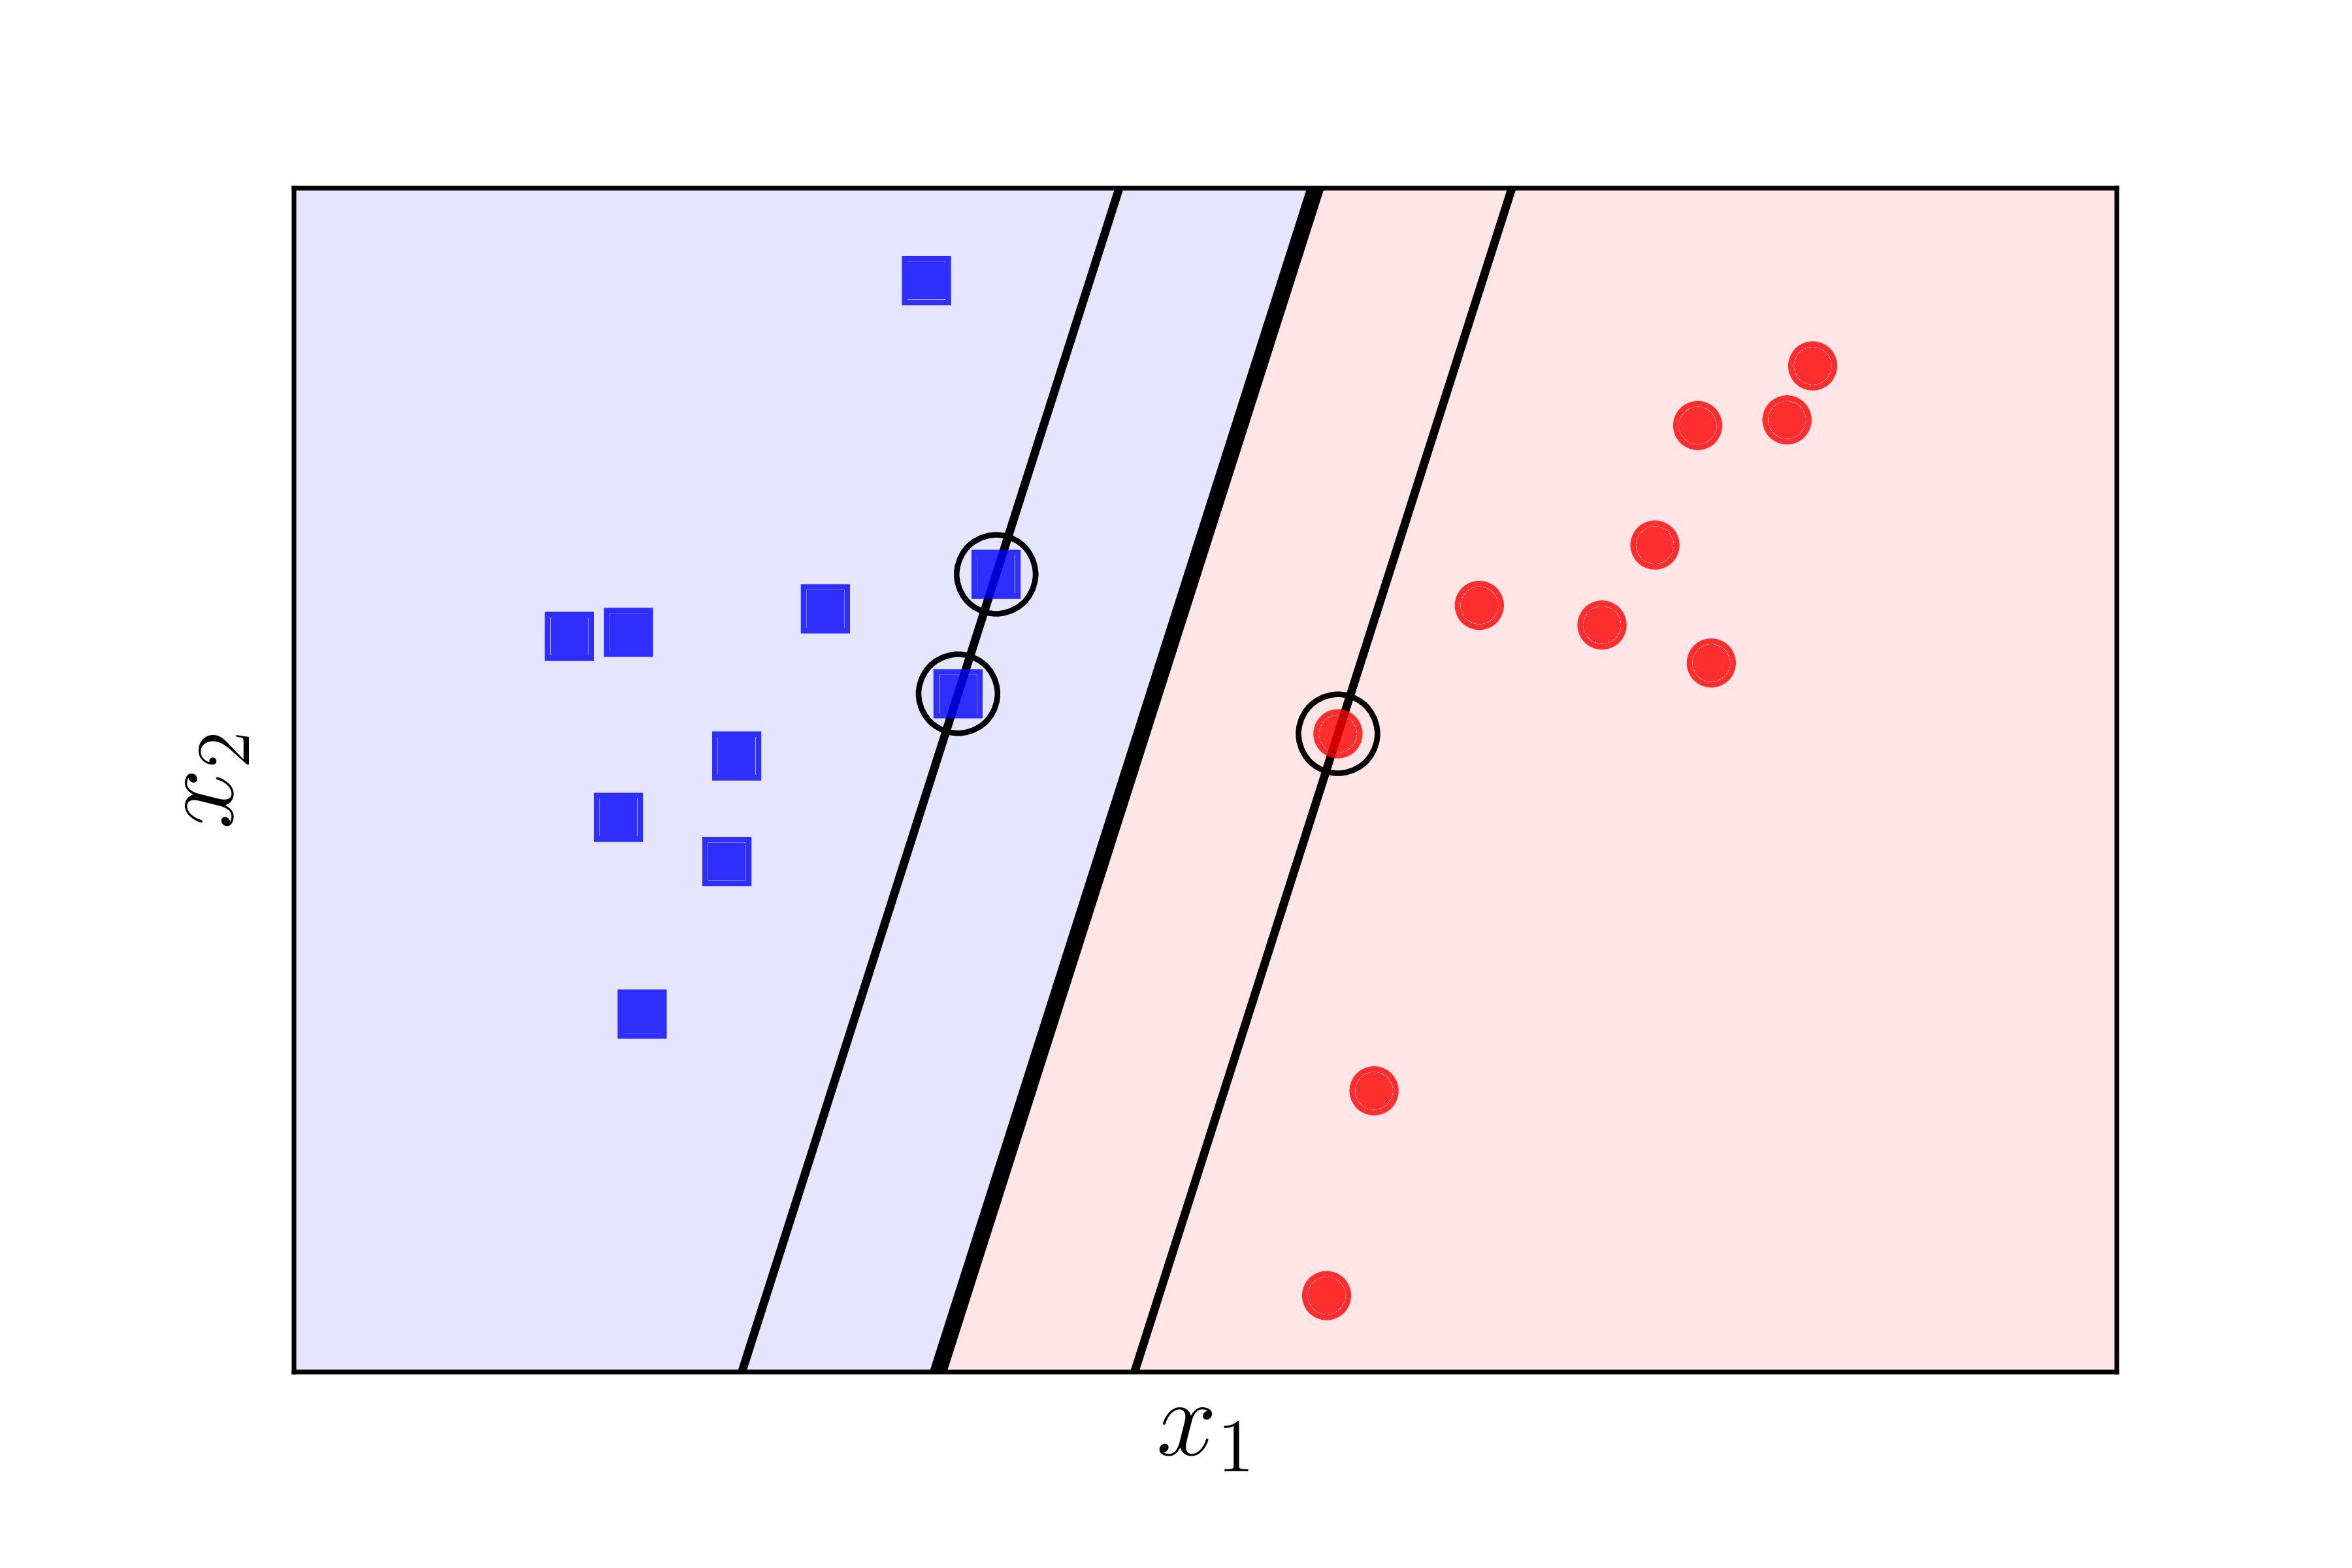
\includegraphics[width=.5\textwidth]{Chapters/09_SupportVectorMachines/19_svm/svm4.png}
    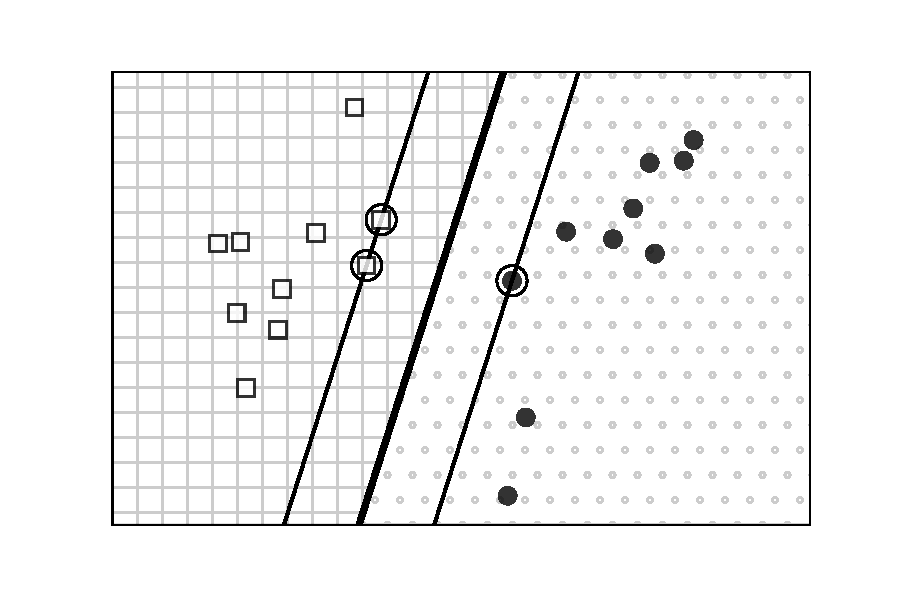
\includegraphics[width=.5\textwidth]{ebookML_src/src/svm/svm4.pdf}
    }
    % \myrule
\end{figure}


Hình vẽ và mã nguồn trong bài có thể được tìm thấy tại \url{https://goo.gl/VKBgVG}.
 

 
\subsection{Tìm nghiệm theo thư viện}
Chúng ta sẽ sử dụng \href{http://scikit-learn.org/stable/modules/generated/sklearn.svm.SVC.html}{\pythoninline{sklearn.svm.SVC}}\footnote{SVC là viết tắt của \textit{bộ phân loại vector hỗ trợ} (support vector classifier).}. Bạn đọc có thể tham khảo thêm thư viện \href{https://www.csie.ntu.edu.tw/~cjlin/libsvm/}{libsvm} được viết trên ngôn ngữ C, có API cho Python và Matlab:

% \newpage 
\begin{lstlisting}[language=Python]
# solution by sklearn 
from sklearn.svm import SVC

model = SVC(kernel = 'linear', C = 1e5) # just a big number 
model.fit(X, y) 

w = model.coef_
b = model.intercept_
print('w = ', w)
print('b = ', b)
\end{lstlisting}
% \newpage 
\kq
\begin{lstlisting}[language=Python]
w =  [[-2.00971102  0.64194082]]
b =  [ 4.66595309]
\end{lstlisting}
 
Kết quả này thống nhất với kết quả tìm được ở mục trước. Có rất nhiều tuỳ chọn cho \pythoninline{SVC}, trong đó có thuộc tính
\pythoninline{kernel}, các bạn sẽ dần thấy trong các chương sau.
 
 
\section{Tóm tắt}
\begin{itemize}
    \item Nếu hai lớp dữ liệu tách biệt tuyến tính, có vô số các siêu phẳng phân chia hai lớp đó.
    Khoảng cách gần nhất từ một điểm dữ liệu tới siêu phẳng này được gọi là
    lề.
     
    \item SVM là bài toán đi tìm mặt phân cách sao cho 
    lề của hai lớp bằng nhau và lớn nhất, đồng nghĩa với việc các điểm dữ liệu có
    một {khoảng cách an toàn} tới mặt phân chia.
     
    \item Bài toán tối ưu trong SVM là một bài toán quy hoạch toàn phương với hàm mục
    tiêu lồi chặt. Vì vậy, cực tiểu địa phương cũng là
    cực tiểu toàn cục của bài toán.
         
    \item Mặc dù có thể trực tiếp giải SVM qua bài toán chính, người ta thường giải bài toán đối ngẫu. Bài toán
    đối ngẫu cũng là một bài toán quy hoạch toàn phương nhưng nghiệm là các vector thưa nên có những
    phương pháp giải hiệu quả hơn. Ngoài ra, bài toán đối ngẫu có những tính chất thú vị sẽ được thảo luận trong các chương tiếp theo.
\end{itemize}
 
% \section{Tài liệu tham khảo }
 
% [1] Bishop, Christopher M. "Pattern recognition and Machine Learning.", Springer  (2006). (\href{http://users.isr.ist.utl.pt/~wurmd/Livros/school/Bishop%20-%20Pattern%20Recognition%20And%20Machine%20Learning%20-%20Springer%20%202006.pdf}{book}) 
 
% [2] Duda, Richard O., Peter E. Hart, and David G. Stork. Pattern classification. John Wiley \& Sons, 2012. 
 
% [3] \href{http://scikit-learn.org/stable/modules/generated/sklearn.svm.SVC.html}{\pythoninline{sklearn.svm.SVC}} 
 
% [4] \href{https://www.csie.ntu.edu.tw/~cjlin/libsvm/}{LIBSVM  --  A Library for SVMs} 
